%% Chapter Template
%
\chapter{Methodology for Data Reshaping} \label{c4} % Main chapter title

\section{Software Structre}

The software structure for the reshaping module is the same as the joining module, refer to Section~\ref{s2.ss} and Fig.~\ref{fig:softflow}.

\section{\textbf{R}}
In the reshaping module, we still use the \textbf{dplyr} and \textbf{tidyr} package. The difference is that in the joining module, we used \textbf{dplyr} more frequently because it provided us with functions to join data sets together. In the reshaping module, \textbf{tidyr} was used more frequently because it contains functions to reshape data sets. 

The idea is the same, but instead of passing information to \textsf{JavaScript} to perform joining animations, we pass in information to perform reshaping animations. They include,

\begin{itemize}
    \item The dimensions and information of the inputted table.
    \item The dimension and information of the resulted table.
    \item The text of the instructional messages to be displayed.
    \item The name and column number of the key columns.
    \item The name and column number of the values columns. 
    \item The corresponding position of where each cell elements within a table goes (in matrix notation).
\end{itemize}

\section{\textbf{dataAnim}}

The reshaping module brings two new functions to the \textbf{dataAnim} package, the \texttt{spread\_anim} function to generate a long to wide animation and the \textttt{gather\_anim} function generates a wide to long animation. \\

The compulsory arguments include the speed of the animation, the data set to apply transformation on, the name of the key and the name of the value. \texttt{gather\_anim} requires an addition argument \texttt{col}, this indicates the columns we wish to reshape on. Below is the help page for \texttt{spread\_anim} shown in Fig.~\ref{fig:spreadhelp} and \texttt{gather\_anim} shown in Fig.~\ref{fig:gatherhelp}.

\begin{figure}[H]
    \centering
    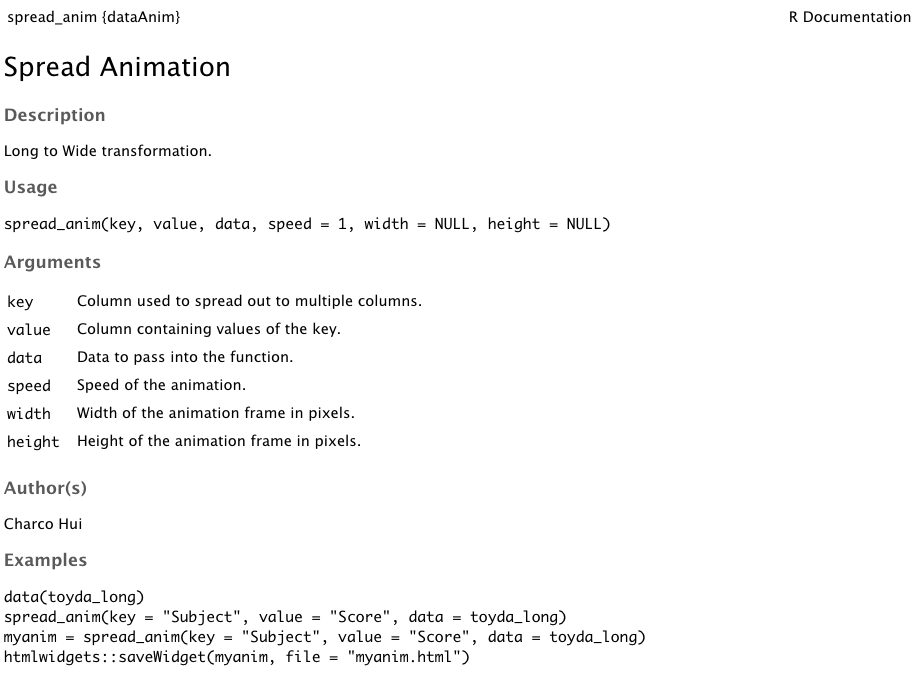
\includegraphics[scale = 0.42]{Masters-Thesis/img/spreadhelp.png}
    \caption{\texttt{spread\_anim} help page}
    \label{fig:spreadhelp}
\end{figure}

\begin{figure}[H]
    \centering
    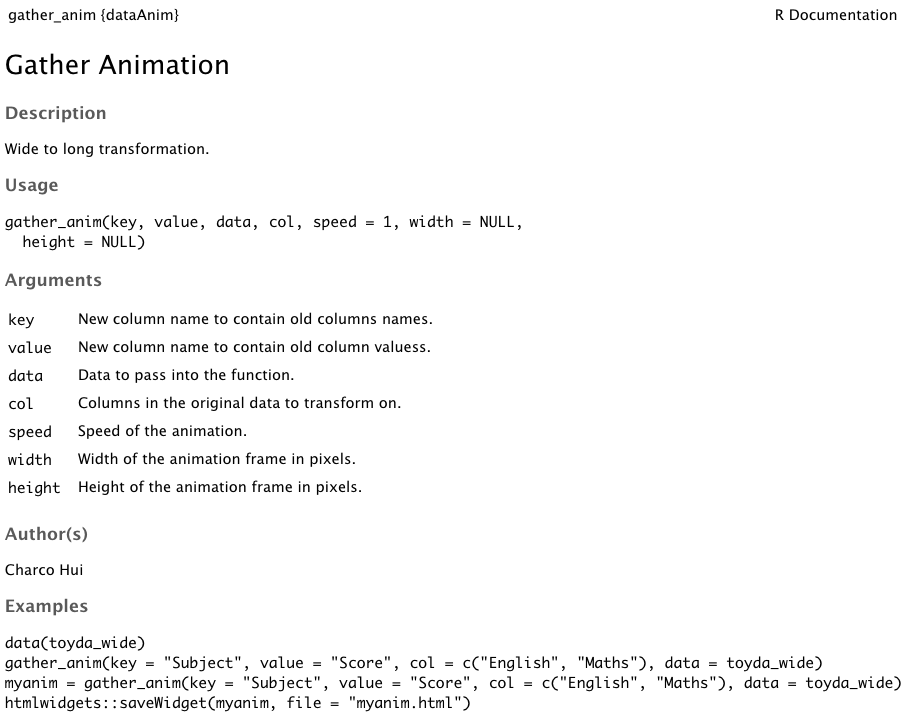
\includegraphics[scale = 0.42]{Masters-Thesis/img/gatherhelp.png}
    \caption{\texttt{gather\_anim} help page}
    \label{fig:gatherhelp}
\end{figure}

\newpage

Discussion of the common arguments:
\begin{itemize}
    \item \texttt{data} is the table to perform reshaping on.
    \item \texttt{speed} allows us to give the user control of the speed of the animation.
    \item \texttt{width} and \texttt{height} are the size of the animation frame in pixels.
\end{itemize}

Discussion of the \texttt{spread\_anim} arguments:
\begin{itemize}
    \item \texttt{key} is the column the user chooses to spread out to multiple columns.
    \item \texttt{value} is the column the that contains the values of the key columns.
\end{itemize}

Discussion of the \texttt{gather\_anim} arguments:

\begin{itemize}
    \item \texttt{key} is the new column name the user wishes to use to contain the old column names.
    \item \texttt{value} is the new column name the user wishes to use to store those values.
    \item \texttt{col} are the columns the user wishes to reshape on.
\end{itemize}
\\

To produce these animation, one method is to use \textbf{Rstudio}. An example of generating a wide to long animation using the \texttt{gather\_anim} in \textbf{Rstudio} is shown in Fig.~\ref{fig:gatherrstudio}.

\begin{figure}[H]
    \centering
    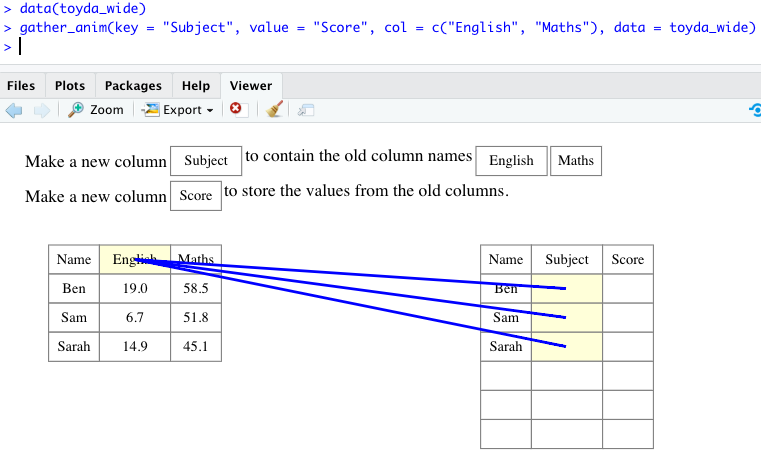
\includegraphics[scale = 0.5]{Masters-Thesis/img/gatherrstudio.png}
    \caption{\texttt{gather\_anim} Example}
    \label{fig:gatherrstudio}
\end{figure}

Another method to generate these animations is to use our \textbf{shiny} interactive dashboard, we will discuss this in Section~\ref{sreshapehtmlwidget}.

\newpage

\section{\textsf{JavaScript} - D3}

In the reshaping module, the use of \textsf{JavaScript} remains the same. However the flow is different. As shown in Fig.~\ref{fig:jsflow2}, the \textsf{JavaScript} program:

\begin{enumerate}
    \item Reads in the instruction from \textsf{R} and passing \textsf{R} objects directly to \textsf{JavaScript} using the \textbf{htmlwidgets} environment. 
    \item Draw the original table given by the user.
    \item Give a brief introduction of the what the animation will be based on.  
    \item Display the structure of the reshaped table. This table will be empty, it is shown to give the user an idea of what the resulted table will look like.
    \item Starts the reshaping animation and display the instructional messages when necessary. 
\end{enumerate}

\begin{figure}[H]
    \centering
    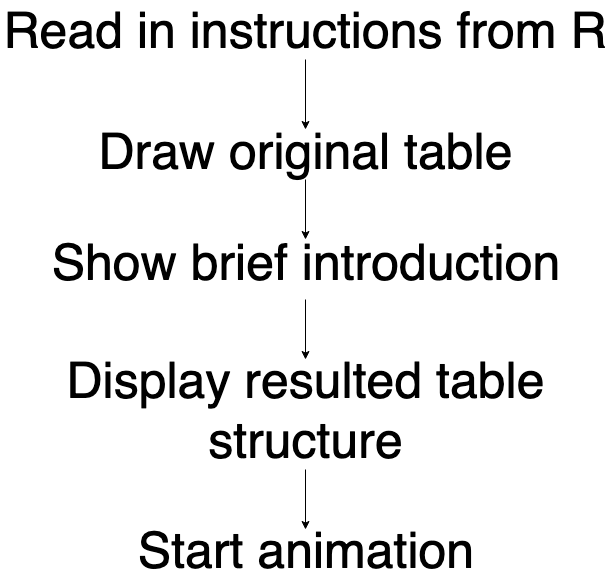
\includegraphics[scale = 0.4]{Masters-Thesis/img/jsflow2.png}
    \caption{\textsf{JavaScript} program flow}
    \label{fig:jsflow2}
\end{figure}


\newpage

\section{\textbf{htmlwidgets} and \textbf{shiny}} \label{sreshapehtmlwidget}
As shown in Fig.~\ref{fig:reshapeshiny}, the \texbf{shiny} interactive dashboard for the reshaping module is different to the joining module. There are three tabs, Tab 1 allow the users to upload their data set in a CSV format, Tab 2 allow users to generate a long to wide animation (Spread) and Tab 3 allow users to generate a wide to long animation (Gather).

\begin{figure}[H]
    \centering
    \begin{tabular}{ccc}
     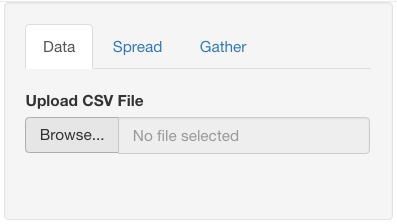
\includegraphics[scale = 0.34]{Masters-Thesis/img/rshinytab1.png} & 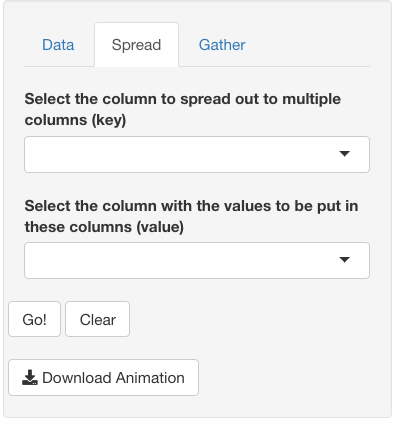
\includegraphics[scale = 0.34]{Masters-Thesis/img/rshinytab2.png} & 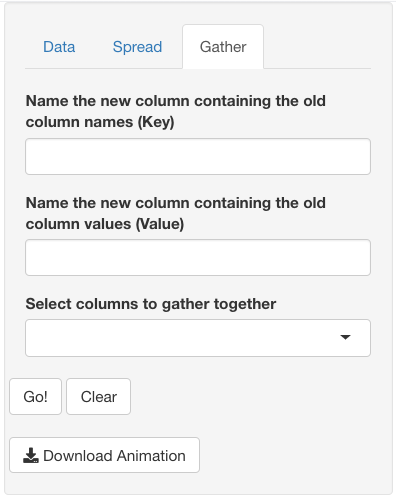
\includegraphics[scale = 0.34]{Masters-Thesis/img/rshinytab3.png} \\
    (a) Tab 1 & (b) Tab 2 & (c) Tab 3 \\[6pt]
    \end{tabular}
    \caption{\textbf{shiny} interactive dashboard (reshape module)}
    \label{fig:reshapeshiny}
\end{figure}

\section{Animation}

In the previous section, some issues with the existing approach of teaching data reshaping were discussed. Some improvements were made to address those issues, with the end goal of making these animations as intuitive as possible. 

The goals of these animations are to:

\begin{itemize}
    \item To show the logic of the data reshaping
    \item Highlight the importance and role of the key and value (columns)
    \item Show the user the relationship between variables in the original table and the resulted table.
    \item Show the underlying process of a wide to long transformation (Spread)
    \item Show the underlying process of a long to wide transformation (Gather)
    \item Show how data are moved between tables
    \item Allow users to download and export the animations.
\end{itemize}